\documentclass{paper}
\usepackage{parskip}
\usepackage{amsmath}
\usepackage{notation}
\usepackage{color}
\usepackage{import}

\usepackage{amsfonts}
\newcommand{\imm}[0]{\text{Imm}}
\newcommand{\maj}{\operatorname{maj}}
\newcommand{\conn}{\mathcal{J}_{\text{conn}}}
\usepackage{hyperref}
\title{Minnesota Research Workshop in Algebra and Combinatorics}
	\author{}
	
	\newcommand{\e}{\mathscr E}
\renewcommand{\d}{\phi}
\newcommand{\redx}[0]{{\color{red}*}}
\newcommand{\W}{\Omega}
\newcommand{\w}{\omega}
\newcommand{\T}{\mathds{T}} % torus
\newcommand{\B}{\mathcal B}
\newcommand{\Sym}{\operatorname{Sym}}
\newcommand{\E}{\bigwedge\nolimits} % Exterior algebra
\newcommand{\PPe}{{\PP{}(\e)}}
	\begin{document}
	\maketitle
	
\section{Positivity of \%-Immanants}
\rightline{\textbf{Sylvester Zhang}}
	\subsection{Introduction}
	Immanants are generalizations of determinants: for any map $f:\mathfrak{S}_n\to \mathbb F$, define the immanant associated to $f$ on the space of $n\times n$ matrices as follows:
	\[\imm_f(a_{ij})=\sum_{\pi\in \mathfrak{S}_n}f(\pi)a_{1\pi(1)}a_{2\pi(2)}\cdots a_{n\pi(n)}\]
	Note that when $f$ is the sign function of permutations, we recover the determinant of square matrices. 
	
	The 2021 REU group of Lu-Ren-Shen-Wang investigated a class of immanants called \%-immanants, which are defined as follows.
	
	\begin{definition}
    For a skew shape $\lambda / \mu$ contained in $n^n $, define
    $$\imm^{\%}_{\lambda/\mu} = \sum_{\sigma \in A} \text{sgn}(\sigma) x_{1, \sigma(1)}x_{2, \sigma(2)}\cdots x_{n, \sigma(n)},$$where $\sigma \in A$ if and only if $(i,\sigma(i)) \in \lambda /\mu$ for all $i$.
    \end{definition}
    In other words, one can calculate a \%-immanants by setting certain corner entries of a matrix to be zero, and take the determinant. For example,
   \begin{equation*}
            \imm^\%_{(4,4,3,3)/(2,1,1)}(x_{ij}) = \det\begin{pmatrix}
                    0 & 0 & x_{13} & x_{14} \\
                    0 & x_{22} & x_{23} & x_{24} \\
                    0 & x_{32} & x_{33} & 0 \\
                    x_{41} & x_{42} & x_{43} & 0
            \end{pmatrix}
        \end{equation*}
 Alternatively, \%-immanants can be defined in terms of permutations. Given a permutation $\omega\in\mathfrak S_n$, its \emph{skew Ferrer matrix} is given by setting entries that are outside of the convex hull of the matrix diagram of $\omega$ to be zero. Let $\lambda/\mu$ be the skew Ferrer shape corresponds to the skew Ferrer matrix of $\omega$, then we define $\imm^\%_\omega:=\imm^\%_{\lambda/\nu}$.  
 
 For example, $\imm^\%_{2413} = \begin{vmatrix}
            0 & \redx & * & * \\
            0 & * & * & \redx \\
            \redx & * & * & 0 \\
            * & * & \redx & 0 \\
        \end{vmatrix}$
        is generated by $2413$, and $\imm^\%_{2413}=\imm^\%_{(4,4,3,3)/(2,1,1) }$.
        
        Following up the REU work of LRSW, we propose to investigate the positivity properties of these \%-immanants.
        
        \subsection{Network positivity}
        A \emph{planer network of order $n$} is a multigraph with more than $2n$ vertices and $2n$ of its vertices are distinguished as boundary: $\{1,2,\cdots,n,1',2',\cdots,n'\}$. For a network $\Gamma$, we can define a matrix $M_\Gamma$ where the entry $(i,j)$ is the weighted sum of all paths from $i$ to $j'$. For example, consider the following network where all edges are directed from left to right.
        \begin{center}
    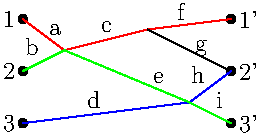
\includegraphics[]{output 20.pdf}
\end{center}
Its corresponding matrix is 
$$\begin{pmatrix} acf & aeh + acg & aei\\ bcf & bcg + beh & bei \\ 0 & dh & di\end{pmatrix}.$$
An immanant $\imm_f$ is said to be network positive if $\imm_f(M_\Gamma)$ has positive coefficient for any planer network $\Gamma$.

LRSW conjectured a condition for which $\%$-immanants are network positive:
\begin{conjecture}[Lu-Ren-Shen-Wang] Signed \%-immanant
$\textup{sgn}(w)\imm_w^{\%}$ is network positive if and only if $w$
	avoids the patterns $1324, 24153, 31524, 426153.$
\end{conjecture} 
\subsection{Schur positivity}
We may further investigate these \%-immanants on Jacobi-Trudi immanants. It is know that Schur functions can be written as the determinant of a matrix. Let $\lambda=(\lambda_1,\cdots,\lambda_n)$ be partition, define the Jacobi-Trudi matrix to be $ (h_{\lambda_{i}+j-i})$, then $s_\lambda=\det(h_{\lambda_{i}+j-i})$. We futher propose the following question of
finding conditions for $w$ such that $\imm_w^\%(h_{\lambda_{i}+j-i})$ is Schur positive.
We suspect that the conditions will be somehow similar to the pattern-avoidance conditions in the network positivity conjecture.

        
\section{Volumes of pattern-avoiding polytopes and Cambrian lattices}\hfill{\textbf{Emily Gunawan}}

The sequence \href{https://oeis.org/A003121}{A003121} counts longest chains in the Tamari lattice; it also counts the number of reduced words in a certain commutation class of the longest permutation. Recently, it was shown by Davis and Sagan that this sequence gives the normalized volume of a certain ``pattern-avoiding polytope'', a subpolytope of the Birkhoff polytope whose vertices are $132$- and $312$- avoiding permutations. Such permutations are known to be $c$-singletons for the symmetric group for a specific Coxeter element $c$. See the most recent comments (2015-2022) in \href{https://oeis.org/A003121}{A003121} by Heinz, Davis, and Gunawan.

For each Coxeter element of the symmetric group, we can define a semi-distributive lattice called a type $A$ Cambrian lattice. The Tamari lattice is a special case of a type $A$ Cambrian lattice. With the exception of the volume of the polytope, all facts above have been generalized to all type $A$ Cambrian lattices.

We propose to generalize Davis' and Sagan's pattern-avoiding polytope results to all type $A$ Cambrian lattices. In particular, we conjecture that the number of longest chains in a type $A$ Cambrian lattice is in fact the volume of a pattern-avoiding polytope. A Polymake computation (thanks to Davis) confirms this conjecture for a so-called bipartite type $A$ Cambrian lattices up to $n=7$.
\section{$P$-Partition Rings and Linear Extensions}
\hfill{\textbf{Sasha Pevzner}}


Let $P$ be a poset on $[n]$. It is a classical enumerative problem to determine the number of \textit{linear extensions} of $P$, that is, the number of permutations $w\in\mathfrak{S}_n$ such that the total ordering $w(1)<w(2)< \cdots <w(n)$ extends the partial order on $P$. For a certain class of posets $P$ called \textit{forests with duplications}, the set of linear extensions of $P$, denoted $\mathcal{L}(P)$, can be counted using the following theorem of F\'eray--Reiner \cite[Theorem 1.1]{FerayReiner}.

\begin{theorem}\label{thm:FR}
Let $P$ be a naturally labelled forest with duplications on $\{1,\ldots,n\}$. Then
\begin{equation}\label{eq: mainEq}
\frac{\sum_{w\in\mathcal{L}(P)} q^{\maj(w)}}{ \prod_{i=1}^n\left(1-q^i\right)} = \frac{ \prod_{\{J_1,J_2\}\in\Pi(P)}\left(1-q^{|J_1|+|J_2|}\right)}{\prod_{J\in\conn(P)}\left(1-q^{|J|}\right)}
\end{equation}
where $\Pi(P)$ denotes the set of pairs $\{J_1,J_2\}$ of connected order ideals in $P$ intersecting nontrivially, $\conn(P)$ is the set of connected order ideals in $P$, and $\maj(w)$ is the major index of the permutation $w$.
\end{theorem}

The left-hand side of (\ref{eq: mainEq}) is the Hilbert series of the \textit{$P$-partition ring} $R_P$, an affine semigroup ring spanned by monomials corresponding to weak $P$-partitions. F\'eray--Reiner showed that $P$ is a naturally labelled forest if and only if $R_P$ has a complete intersection presentation. In this case, the minimal free resolution of $R_P$ is a Koszul complex. 

When $R_P$ is not a complete intersection, one can still form the Koszul complex on the generators of its defining ideal and investigate its homology. If it is sufficiently well behaved, then (\ref{eq: mainEq}) will become an inequality with the lefthand side being the upper bound. The goal of this project is to quantify when this occurs.


\textbf{Credit}: Thanks to Vic for introducing me to this problem!

\bibliographystyle{abbrv}
\bibliography{biblio}
\section{Trip Permutations for Unreduced Plabic Graphs}

\hfill{\textbf{Sunita Chepuri}}


Plabic graphs give parametrizations of positroid cells in the totally nonnegative Grassmannian: as the weights vary, the image of the network under Postnikov's boundary measurement map varies over the entire cell. If a plabic graph is reduced, we can determine  which positroid cell it parametrizes by computing the trip permutation.  It remains an open question how to determine this for an unreduced plabic graph.

\section{Toric Varieties and Problems in Algebraic Combinatorics}
\hfill\textbf{Mahrud Sayrafi}
\subsection{Introduction}

Toric varieties are algebraic varieties with an intrinsic combinatorial structure, making them a prime crucible for interesting examples in algebraic geometry. At the same time, there are interesting problems in algebraic combinatorics whose solutions involve toric varieties. For instance, Stanley used toric varieties and the hard Lefschetz theorem to prove necessity of a condition, conjectured by McMullen, for a vector of integers to be the $f$-vector of a simplicial convex polytope \cite{Stanley80}.

% \section{Toric Varieties}

% In this section we briefly recall the terminology for normal toric varieties and give a number of key running examples of toric varieties. For an in depth exposition see \cite{CLS2011} and \cite{Fulton1993}.

The structure of an \emph{affine toric variety} can be characterized by a \emph{strongly convex rational cone}. Concretely, let $N$ be a lattice in $\ZZ^n$ and $\sigma$ a cone in $N$, then the dual cone $\sigma^\vee$ in $M=\Hom_\ZZ(N, \ZZ)$ is the set of vectors in $M\otimes_\ZZ\RR$ with non-negative inner product on $\sigma$. This gives a commutative semi-group \( S_\sigma = \sigma^\vee \cap M = \{ \eta \in M : \eta(\nu) \geq 0 \text{ for all } \nu\in\sigma \}, \) and an open affine toric variety \( U_\sigma = \Spec\;\CC[S_\sigma] \) corresponding to its group algebra.
The gluing data for a general toric variety comes from a \emph{fan} of cones.

\begin{definition}
  A \emph{fan} $\Delta$ of strongly convex polyhedral cones in $N_\RR = N\otimes_\ZZ\RR$ is a set of
  rational strongly convex polyhedral cones $\sigma\in N_\RR$ such that:
  \begin{enumerate}
  \item each face of a cone in $\Delta$ is also a cone in $\Delta$;
  \item the intersection of two cones in $\Delta$ is a face of each of the cones.
  \end{enumerate}
\end{definition}

\begin{table}[h]
\centering
\begin{tabular}{@{\extracolsep{1ex}} ccccc} % {c|*{4}{c}}
%    $\PP1$
    $\PP2$
  & $\PP1\times\PP1$
  & $\FF_1$ % Hirzebruch
  & $\mathrm{Bl}_x(\FF_1)$
  & $\mathrm{dP}6$
  \\ \hline
%    \def\svgwidth{75px} \import{./images/}{PP1.pdf_tex}
    \def\svgwidth{75px} \import{./images/}{PP2.pdf_tex}
  & \def\svgwidth{75px} \import{./images/}{PP1xPP1.pdf_tex}
  & \def\svgwidth{75px} \import{./images/}{H1.pdf_tex}
  & \def\svgwidth{75px} \import{./images/}{BlF1.pdf_tex}
  & \def\svgwidth{75px} \import{./images/}{dP6.pdf_tex}
\end{tabular}
\vspace{15pt}
\caption{Fans of the five smooth toric Fano surfaces}\label{tab:toric-examples}
\end{table}

With this information in hand, a normal toric variety $X$ is fully characterized as follows: given a fan
$\Delta$, $X(\Delta)$ is assembled by gluing the affine toric subvarieties $U_\sigma$ for each $\sigma\in\Delta$.
If every cone $\sigma\in\Delta$ is generated by a subset of a $\ZZ$-basis of $N$ then $X$ is smooth, and
it is simplicial if every cone is generated by a subset of an $\RR$-basis of $N_\RR$.
% Projective if the fan is complete; i.e. all points are in a maximal cone

\iffalse
Let $\Delta(i)$ denote the set of $i$-dimensional cones in $\Delta$. A 1-dimensional cone $\rho\in\Delta(1)$ is referred to as a \emph{ray} and corresponds to an irreducible $\T$-invariant \emph{Weil divisor} $D_\rho$ on $X$.
% Recall that a divisor on a variety $X$ is an element of the free abelian group generated by the subvarieties of
% codimension one, denoted $\Div X$.
Hence we identify $\Div X = \ZZ^{\Delta(1)}$ and define $\CDiv X$ to be the subgroup of $\T$-invariant
\emph{Cartier divisors} on $X$. To any Cartier divisor $D$ on a normal variety $X$ we can associate an
\emph{invertible sheaf} $\l = \o_X(D)$ which is a locally free sheaf of sections of a \emph{line bundle}
$L \to X$. Isomorphism classes of such line bundles on $X$ define the \emph{Picard group $\Pic X$}.
% with tensor product as the group operation.
% Two divisors are \emph{linearly equivalent}, denoted $D \sim D'$, if $D - D'$ is a \emph{principal divisor}.

The relationship between these groups is captured in a commutative diagram of $\ZZ$-modules
% https://q.uiver.app/?q=WzAsMTAsWzAsMCwiMCJdLFsxLDAsIk0iXSxbMiwwLCJcXENEaXYgWCJdLFszLDAsIlxcUGljIFgiXSxbNCwwLCIwIl0sWzAsMSwiMCJdLFsxLDEsIk0iXSxbMiwxLCJcXERpdiBYIl0sWzMsMSwiQV97bi0xfShYKSJdLFs0LDEsIjAiXSxbMCwxXSxbMSwyXSxbMiwzXSxbMyw0XSxbNSw2XSxbNiw3XSxbNyw4XSxbOCw5XSxbMSw2LCIiLDEseyJsZXZlbCI6Miwic3R5bGUiOnsiaGVhZCI6eyJuYW1lIjoibm9uZSJ9fX1dLFsyLDcsIiIsMSx7InN0eWxlIjp7InRhaWwiOnsibmFtZSI6Imhvb2siLCJzaWRlIjoidG9wIn19fV0sWzMsOCwiIiwxLHsic3R5bGUiOnsidGFpbCI6eyJuYW1lIjoiaG9vayIsInNpZGUiOiJ0b3AifX19XV0=
\begin{equation}\label{eq:toric-div}
\begin{tikzcd}[row sep=small]
	0 & M & {\CDiv X} & {\Pic X} & 0 \\
	0 & M & {\Div X} & {A_{n-1}(X)} & 0,
	\arrow[from=1-1, to=1-2]
	\arrow["\mathrm{div}", from=1-2, to=1-3]
	\arrow[from=1-3, to=1-4]
	\arrow[from=1-4, to=1-5]
	\arrow[from=2-1, to=2-2]
	\arrow[from=2-2, to=2-3]
	\arrow[from=2-3, to=2-4]
	\arrow[from=2-4, to=2-5]
	\arrow[Rightarrow, no head, from=1-2, to=2-2]
	\arrow[hook, from=1-3, to=2-3]
	\arrow[hook, from=1-4, to=2-4]
\end{tikzcd}
\end{equation}
% isomorphisms when X is smooth
% injective because $\Delta(1)$ spans $N_\RR$ by assumption.
% TODO: \beta is the quotient map, give it a better name? it gives the \Pic X grading on S
where \( \mathrm{div}(m) = \sum_\p \langle m, n_\p \rangle D_\p \) with $n_\p \in N$ the generator of
$\p\subset N_\RR$ computes the orders of poles and zeros along the divisors $D_\p$.
See \cite{Cox95} or \cite[Ch.II \S6]{Hartshorne1977} for further context.

\begin{definition} For a toric variety $X$, the \emph{homogeneous coordinate ring} is the polynomial ring
  \( S = \Cox X = \CC[x_\p : \p\in\Delta(1)] \) where each divisor $ D = \sum_\p a_\p D_\p $ is represented by
  a monomial $ x^D = \prod_\p x_\p^{a_\p} $ with $ \deg(x^D) = [D] \in A_{n-1}(X) $.
  % Chow group of Weil divisors modulo rational equivalence

  The data of the fan determine an exceptional set $Z(\Delta) \subset \CC^{\Delta(1)}$ which is the zero set of
  the \emph{irrelevant ideal} \( B(\Delta) = \langle \hat x_\sigma : \sigma\in\Delta \rangle \)
  generated by the square-free monomials $\hat x_\sigma = \prod_{\p\not\subset\sigma} x_\p$.
  \end{definition}
\fi

\subsection{Problems}

There are various other combinatorial descriptions of toric varieties (e.g., from a lattice polytope), so many combinatorial problems can be translated into problems about existence or classification of toric varieties (or even vector bundles on them). Here are two potentially interesting examples:

\subsubsection{Classify smooth projective toric varieties with few generators}

Two toric varieties $X_\Delta$ and $X_{\Delta'}$ are isomorphic if there is a unimodular transformation of the lattice $N$ which maps $\Delta$ to $\Delta'$ and which induces an isomorphism of the simplicial complexes associated to them. In \cite{Kleinschmidt88}, Peter Kleinschmidt classified smooth projective toric varieties of Picard rank 2 but with arbitrary dimension by studying the unimodular transformations between the lattices. This classification essentially says that such toric varieties correspond to $2 \times(r + s + 1)$ matrices:

\[
\begin{pmatrix}
  1 & 1 & \cdots & 1 & 0 & a_1 & a_2 & \cdots & a_s \\
  0 & 0 & \cdots & 0 & 1 & 1   & 1   & \cdots & 1
\end{pmatrix}
\]

The question is, to what extend can we generalize this to toric varieties (perhaps with some added adjectives, as desired) of Picard rank 3.

%\begin{example}\label{eg:root-system} Toric Variety from a Root System
% https://arxiv.org/abs/0911.3607v4 & https://arxiv.org/abs/0912.2898
%\end{example}

\subsubsection{Toric varieties from root systems}


%%%%%%%%%%%%%%%%%%%%%%%%%%%%%%%%%%%%%
\nocite{*}
\bibliographystyle{amsalpha}
\bibliography{references-5}
\section{TBD}
\hfill\textbf{Esther Banaian}
	

\end{document}